\chapter{Project Management}
\label{ch:project-management}
% https://warwick.ac.uk/fac/sci/dcs/teaching/material/cs310/components/final/marking/management
% https://warwick.ac.uk/fac/sci/dcs/teaching/material/cs310/reusingcontent

\section{Specification}
\label{sec:specification}

At the start of the project, a set of MoSCoW prioritised \cite{CaseMethodFastTrack} requirements were created, which fully defined concrete goals for the project. These are included in Appendix \ref{sec:project-requirements}. These fixed requirements gave the project a clear overall goal from a very early stage, and helped adopt good planning and development methodologies. 

\section{Organisation}
\label{sec:organisation}

Good organisation is critical to the success of any project. To guarantee the success of this project, I maintained a strong focus on organisation from the start of the specification, for example by having regular, minuted, meetings with my project supervisor, and setting aside regular blocks of time in my week to make progress towards timelined goals.

\subsection{Project plan}
\label{ssec:organisation-plan}

One important aspect of project organisation is having a robust plan. Following the creation of the project requirements, I created a Gantt chart to set a timeline for their completion, shown in Figure \ref{fig:diss_gantt_spec_2}:

\begin{figure}[ht]
    \centering
    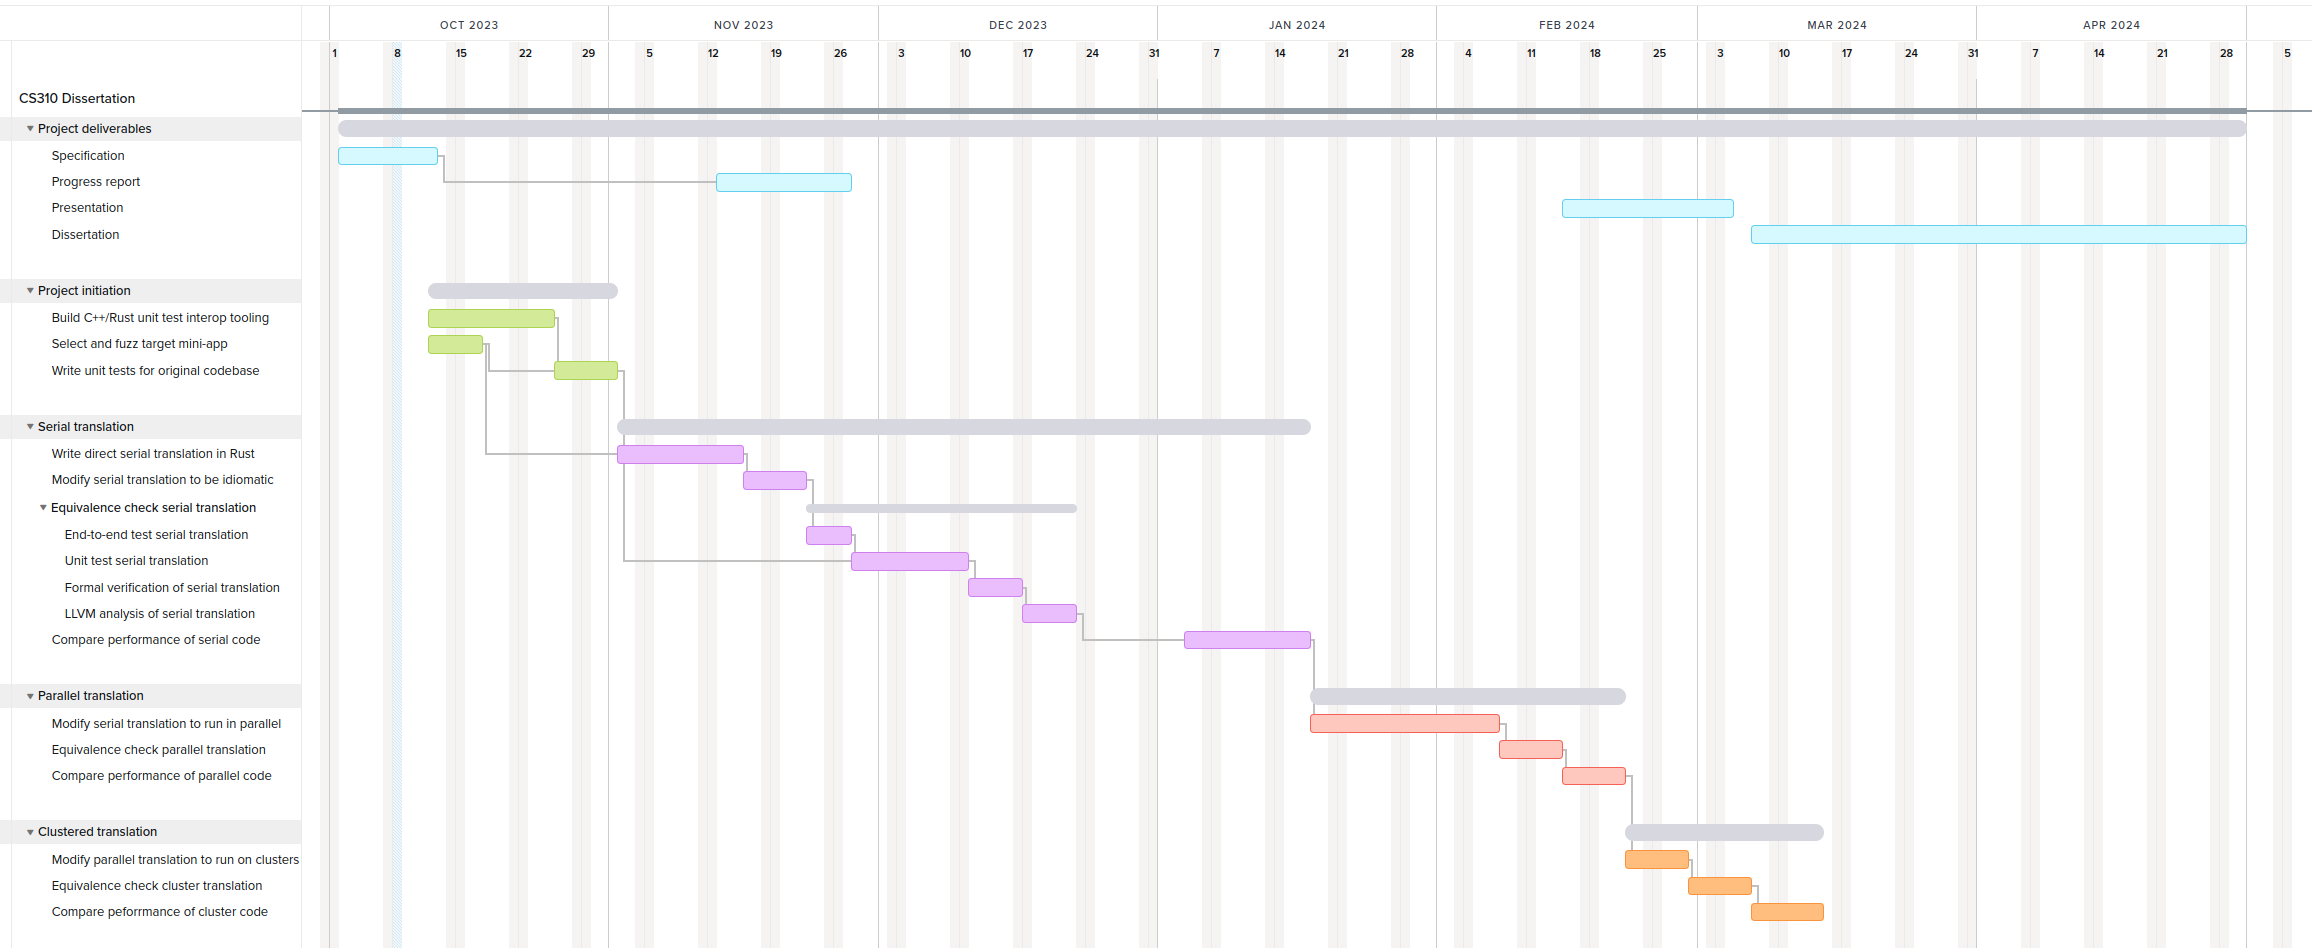
\includegraphics[width=\textwidth]{images/6_project_management/diss_gantt_spec_2.png}
    \caption{Gantt chart of the proposed project timetable, showing each of the objectives and the dependencies between them.}
    \label{fig:diss_gantt_spec_2}
\end{figure}

As discussed in the development methodology section \ref{ssec:organisation-methodology}, I followed an Agile methodology to undertake this project. One key benefit of this project was adaptability to change based on new information or supervisor discussion (following the agile manifesto: ``Responding to change over following a plan'' \cite{beckManifestoAgileSoftware2001}). 

When approaching the half-way point of the project and writing the progress report, I had made very strong progress towards the project objectives, with a working implementation of the Rust translation of the HPCCG \acrshort{mini-app} completed ahead of schedule. As a result of this new information, following discussion with my supervisor, I chose to modify my project plan to include the translation of a second, larger \acrshort{mini-app}, called MiniMD \cite{osti_1231191}. During the Christmas break, I investigated the MiniMD codebase and build system, and found that it presented unforeseen challenges, for example a build process which involved a Makefile manually expanding C++ macros. This build process did not map well into modern build systems like CMake, nor Rust's procedural macro system. As a result of this, again following discussion with my supervisor, I chose to return to the original project plan, with the stretch goal of translating the MPI component of HPCCG. This allowed me to extend the scope of the assessment of Rust's capability as a language for \acrshort{HPC}, and gave me time to build the HPC MultiBench tool, which was not initially planned. These significant changes would be very difficult following a plan-based methodology, such as waterfall -- but were possible through Agile, and resulted in a better project outcome, informed by experience learnt in the process.

% The final version of the project timeline is shown as a Gantt chart in Figure \ref{}:
% NOTE: Consider making final Gantt chart

In summary, creating and following a project plan from the start of the project, whilst being empowered to change it as required, contributed strongly to the success of this project.

\subsection{Development methodology}
\label{ssec:organisation-methodology}

In 2001, a group of seventeen leaders in the field of software engineering published ``The Manifesto for Agile Software Development'' \cite{beckManifestoAgileSoftware2001}. This proposed four key principles to consider during software development:

\begin{itemize}
    \item Individuals and interactions over processes and tools
    \item Working software over comprehensive documentation
    \item Customer collaboration over contract negotiation
    \item Responding to change over following a plan
\end{itemize}

These ideas spawned many software development frameworks, such as Kanban, Scrum, and Lean. This project is well-suited to an Agile approach, since it has a significant software development, but cannot easily be planned in full ahead of time, as new information affecting the project plan is generated throughout by the research component.

I chose to use a variant of the Scrum methodology, as it is simple to implement -- allowing me to focus on the technical work in the project, and I already had experience using it from my year in industry. This manifested itself as weekly sprints, which start and end with a supervisor meeting. Prior to these meetings, an agenda was prepared, which usually included talking points about the work done in that week, and any questions relating to the project. This was helpful as it ensured that no important points were forgotten during the meeting, and stimulated the conversation. After each meeting, summary minutes of the meeting were written up and uploaded to Tabula. This helped formalise the outcome of the meeting, generating a deliverable to allow the review of what happened in each sprint at the end of the project. A diagram of this process is shown in Figure \ref{fig:excalidraw_agile}.

\begin{figure}[h]
    \centering
    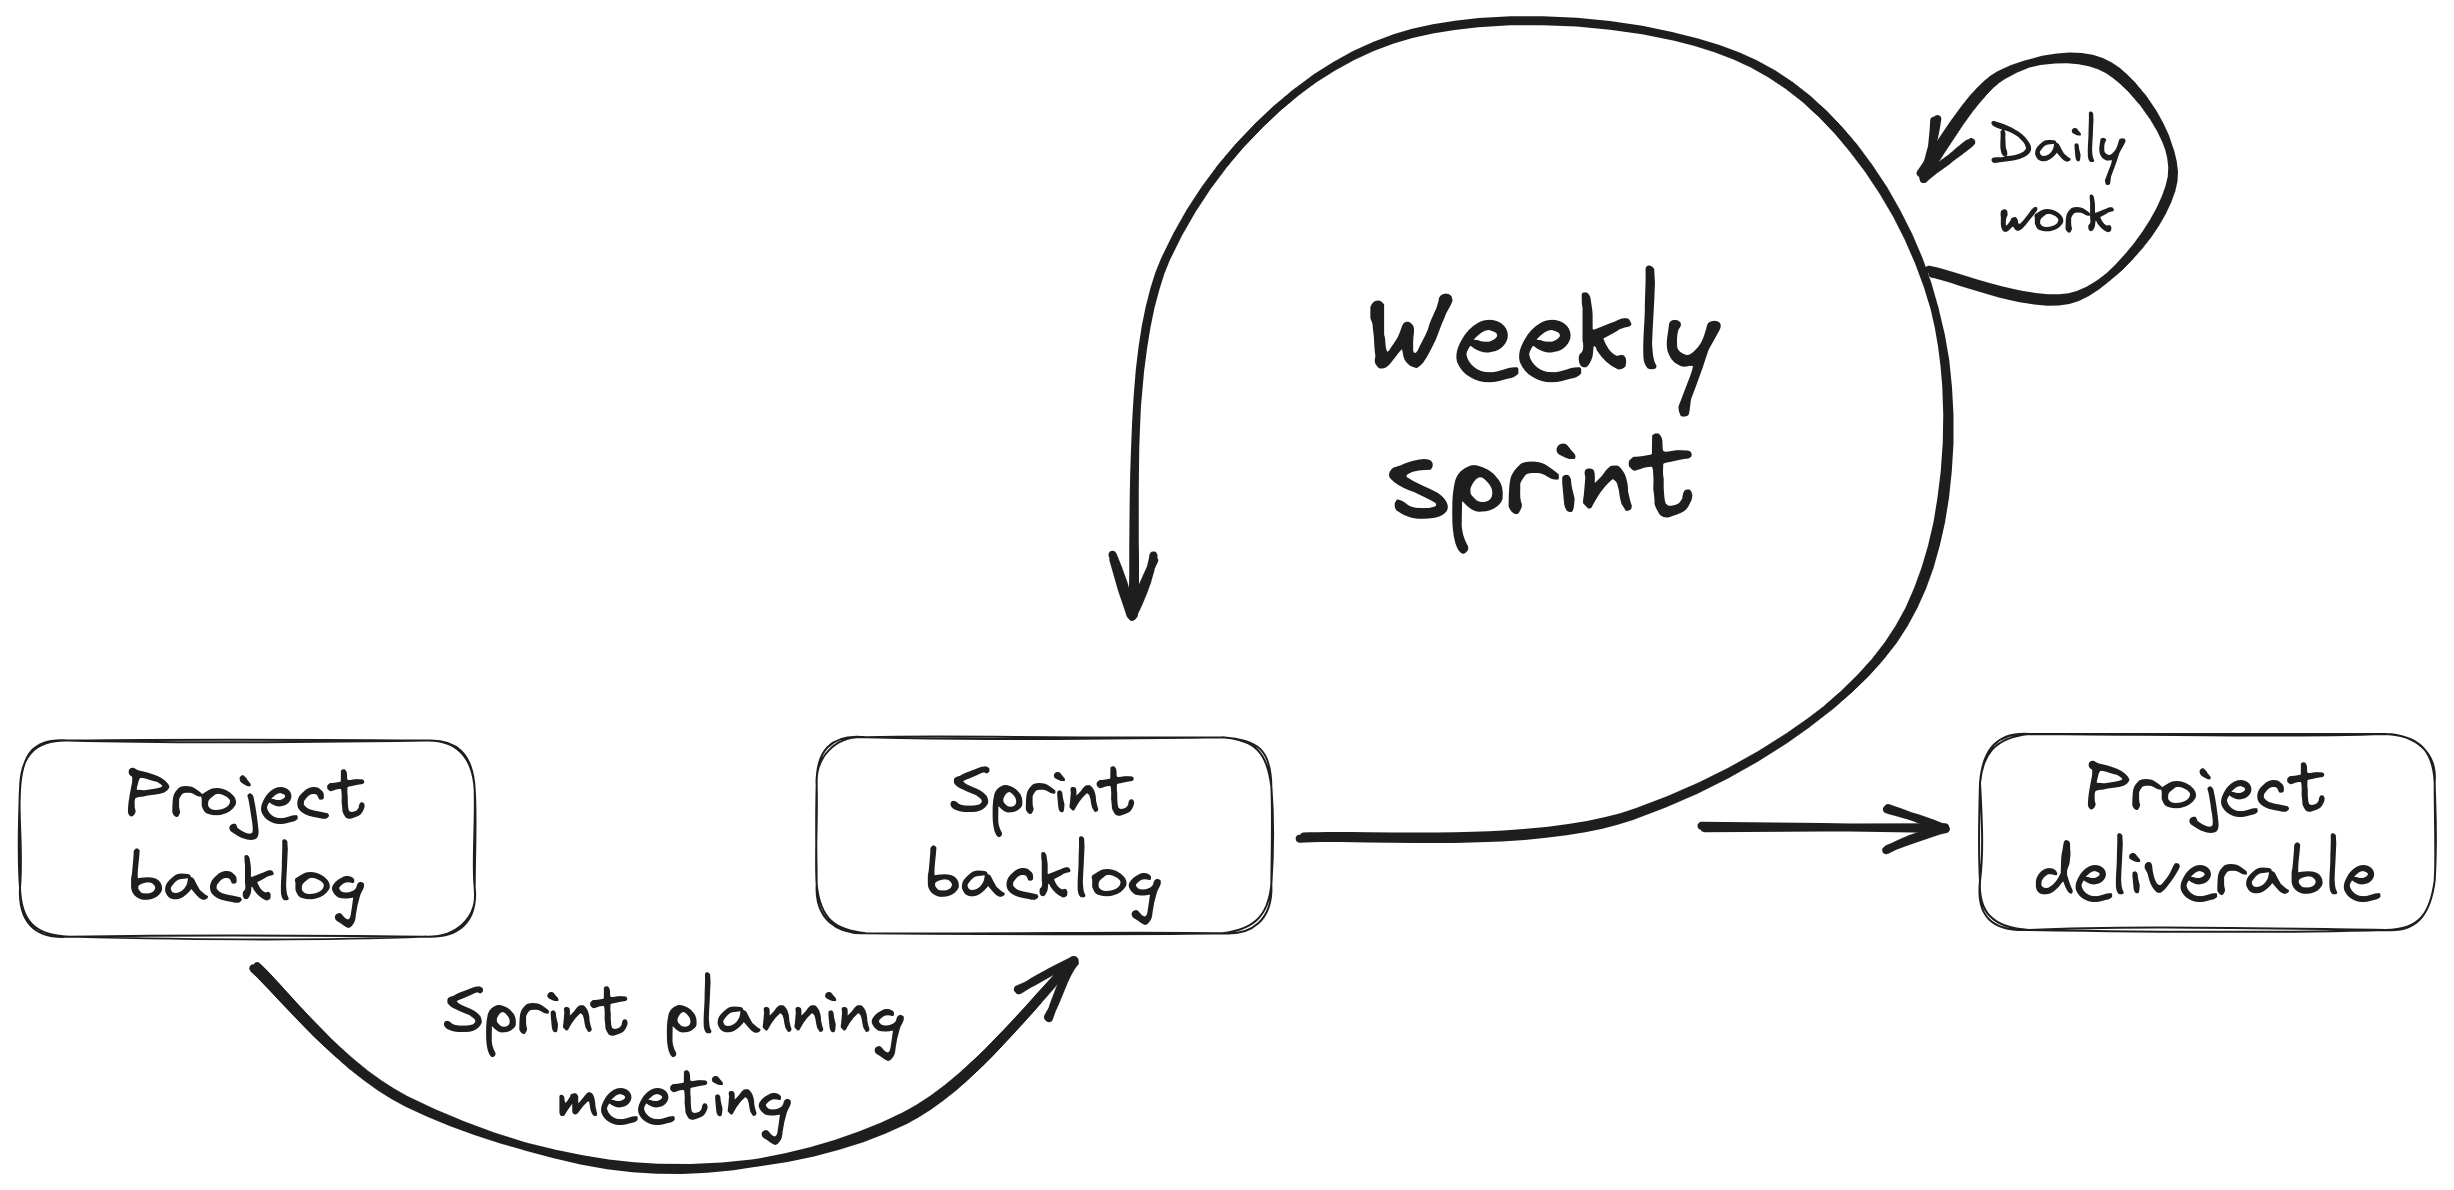
\includegraphics[width=0.75\textwidth]{images/6_project_management/excalidraw_agile.png}
    \caption{Typical workflow for the Scrum flavour of Agile development.}
    \label{fig:excalidraw_agile}
\end{figure}

This decision to manage the project with an agile methodology has yielded many benefits, including:

\begin{itemize}
    \item Being goal-oriented with respect to achieving the objectives laid out at the start of the project
    \item Being motivated to immediately write code and deliver working software for each sprint
    \item Being empowered to adapt the initial plan, based on any new information and ongoing discussions during supervisor meetings
\end{itemize}

\subsection{Software tools}
\label{ssec:software-tools}

This project heavily leveraged \texttt{git} in combination with a private GitHub repositories. All source code, from helper scripts to software products, are tracked in \texttt{git}. Using \texttt{git} for source control management allowed syncing work across DCS, SCRTP, and personal machines, and reviewing and restoring to work done in the past.

A significant aspect of the project was developing software, resulting in two major software products:

\begin{enumerate}
    \item The translated \acrshort{mini-app} code -- necessarily written in Rust.
    \item The HPC MultiBench tool -- written in Python for high-velocity development.
\end{enumerate}

For this software development, I followed the GitHub flow development workflow \cite{GitHubFlow} which leverages lightweight \texttt{git} branching to develop atomic features. For the software development components, I used GitHub actions to run CI/CD workflows \cite{WhatCICD} such as linters and test harnesses to guarantee code quality and correctness.

Long-format text was written in \LaTeX\ using Overleaf\cite{OverleafOnlineLaTeX}, and also tracked in \texttt{git} via Overleaf's integration with GitHub for linear commit histories. In addition to this, I used Zotero \cite{ZoteroYourPersonal} to manage citations, which again supports an integration with Overleaf.

\subsection{Responding to unforeseen issues}
\label{ssec:organisation-unforeseen-issues}

As discussed in the previous section, \ref{ssec:organisation-methodology}, following an Agile methodology empowered the project to be flexible to change, allowing the original plan to be adapted based on new information or ongoing supervisor discussions. A concrete example of this is the development of the HPC MultiBench tool. Its development was not an explicit project requirement enumerated in the specification, but following identification of a need and supervisor discussion, it was included as part of the project to facilitate performance analysis. This successful deviation from the initial project plan also supports the fact that the chosen methodology would have been robust against major unforeseen issues, had any occurred.

In the project specification, a Risk Matrix characterising possible issues was generated, as shown in Table \ref{tab:risk_matrix}, included in Appendix \ref{sec:risk-matrix-appendix}. Of these identified possible risks, the only one which manifested itself was compute resources becoming busy, which is consistent with it having the highest estimated likelihood. This had a low impact on the project progress, as I had access to two resources (both \texttt{kudu} on DCS and \texttt{Avon} on SCRTP), and could switch to other tasks whilst waiting for long jobs to complete.

\section{Effort and motivation}
\label{sec:effort-and-motivation}

I believe this project could be described as high effort through deeply consistent work. In the first term, I had no timetabled lectures nor seminars on Fridays, so set them aside as a time to work exclusively on the project. This allowed me to avoid incurring the cost of context switching to other activities. As a result of this, I was able to make strong progress, completing the translation and parallelisation objectives ahead of schedule. In the new year, I suggested and undertook a challenge along with a group of friends to make a project-related \texttt{git} commit every day during the month of January (``proj-anuary'', a portmanteau of project and January). I then chose to continue this for the entirety of the second term of this academic year, as shown in Figure \ref{fig:github_year_long_contributions}.

\begin{figure}[H]
    \centering
    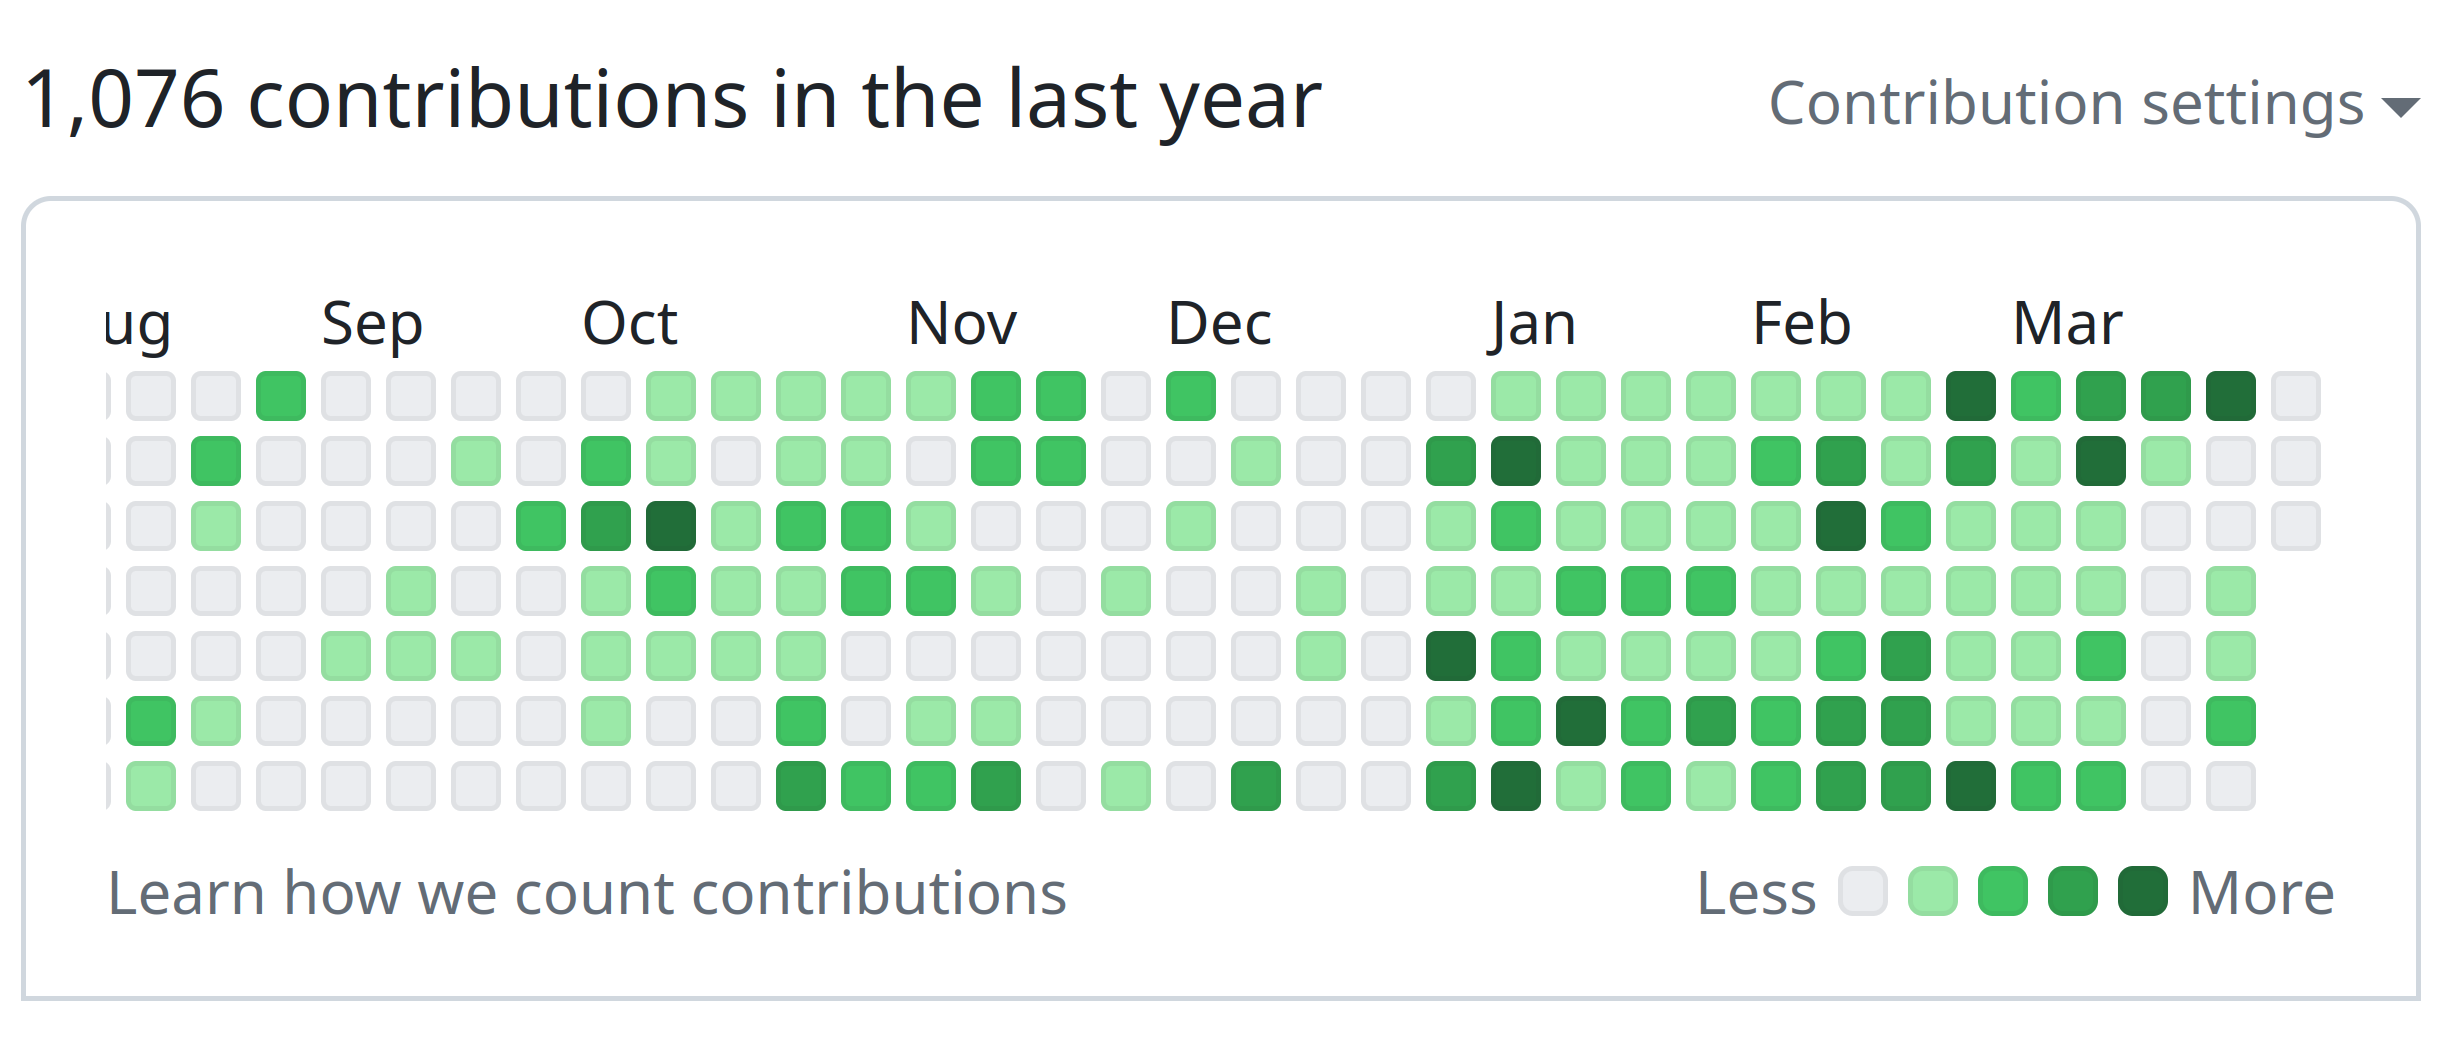
\includegraphics[width=0.75\textwidth]{images/6_project_management/github_year_long_contributions.png}
    \caption{The author's GitHub contributions over the past academic year. Commits from January 1\textsuperscript{st} to March 18\textsuperscript{th} form an unbroken consecutive streak of 78 days.}
    \label{fig:github_year_long_contributions}
\end{figure}

This consistent approach to project progression paid great dividends, with even stronger progress being made in the second term than the first. This included successfully completing the stretch goal of running Rust code across clustered compute resources using MPI, and building the HPC MultiBench tool for generalised performance analysis of software executed via Slurm.

\section{Legal, social, ethical, and professional issues}
\label{sec:legal-social-ethical-professional-issues}

At the start of the project, any legal, social, ethical, and professional issues that might relate to the project were identified. 

Firstly, a small number of legal issues were identified as relating to the project, largely relating to software licensing. Since \acrshort{HPC} is an active field of development in industry, some libraries or tools may have restrictive licences, so care was taken when picking and using tools to conform to the terms of their licences. Additionally, when identifying possible legal issues in the specification, it was noted that some \acrshort{mini-app}s in the Mantevo suite are based on simulations of experiments in nuclear physics, so working with them might require special care to conform to relevant UK law. However, this issue was mitigated by selecting to examine the HPCCG \acrshort{mini-app} \cite{herouxHPCCGSolverPackage2007}, which is instead based on methods of conjugate gradients solving linear systems \cite{hestenesMethodsConjugateGradients1952}.

Secondly, a level of professionalism is required for all projects. This project does not necessitate any professional considerations above basic norms, such as making meaningful commit messages, or writing well documented and maintainable code.

% Finally, since this project does not use human-generated data (for example data from surveys), nor is it creating a product humans directly use, it does not have any notable ethical nor social considerations. This was verified by following the flowchart on the \href{https://warwick.ac.uk/fac/sci/dcs/teaching/ethics}{ethical consent page of the project website}. % NOTE: Could argue that shift to building HPC multibench requires social considerations, but I don't think that it does
Finally, since this project does not use human-generated data (for example data from surveys), it does not have any notable ethical nor social considerations. This was verified by following the flowchart on the \href{https://warwick.ac.uk/fac/sci/dcs/teaching/ethics}{ethical consent page of the project website}.

Due to the importance of these categories of issues, they were reviewed again for any changes at the midpoint of the project when writing the progress report, and yet again at the end when writing the final report. Since the project remained broadly fixed in scope, no additional issues were identified at either of these points.

In summary, this project carefully considered all relevant legal, social, ethical, and professional issues pertaining to the project, which constitutes a critical component of any successful project.

